%\documentclass[preprint,authoryear,12pt]{elsarticle}
\documentclass[final,authoryear,5pt,times,twocolumn]{elsarticle}

\usepackage{amssymb}
\usepackage{amsmath}
\usepackage{booktabs}
\usepackage{textcomp}

\newcommand{\vect}[1] %vector notation
{{\bf {#1}}}
\newcommand{\npoly}{$n$-polytope}
\newcommand{\citepp}[4] %double parenthesis cite
{(\citealp[{#1}]{{#2}}; \citealp[{#3}]{{#4}})}
\newcommand{\bpm}{\begin{pmatrix}} %for matrix notation
\newcommand{\epm}{\end{pmatrix}}

\journal{Journal of Process Control}

\begin{document}

%% ==== HEAD ====
\begin{frontmatter}

\title{A Systematic Approach to Model Predictive Controller Constraint Handling: Rigorous Geometric Methods}

\author{Andr\'e H. Campher}
\ead{ahcampher@tuks.co.za}

\author{Carl Sandrock\corref{cor1}}
\ead{carl.sandrock@up.ac.za}

\cortext[cor1]{Corresponding author\\Tel.: +27 12 420 2197; Fax: +27 12 420 5048}

\address{Department of Chemical Engineering, University of Pretoria, Pretoria 0001, South Africa}

\begin{abstract}
The models used by model predictive controllers (MPCs) to predict future outcomes are usually unconstrained forms like impulse or step responses and discrete state space models. 
Certain MPC algorithms allow constraints  to be imposed on the inputs or outputs of a system; but they may be infeasible as they are not checked for consistency via the process model. 
Consistent constraint handling methods -- which account for their interdependence and disambiguate the language used to specify constraints -- would therefore be an attractive addition to any MPC package.

A rigorous and systematic approach to constraint management is proposed, building on the work of \citet{vinsonartoi} in interpreting constraint interactions. 
The method focuses on linear steady-state system models, and provides routines to obtain the following information; effects of constraint changes on the corresponding input or output constraints, feasibility checks for constraints, constraint-type information, specification of constraint-set size and optimal fitting of constraints within the desirable input or output space.

Mathematical rigour and unambiguous language for identifying constraint types were key design criteria. 
The application of the method is illustrated for a laboratory scale distillation column running commercial MPC packages.
\end{abstract}

\begin{keyword}
constraint handling \sep model predictive control \sep geometric methods \sep operability index
\end{keyword}

\end{frontmatter}

%\linenumbers


%% ==== BODY ====
\section{Introduction}\label{sec:intro}
The ability of some MPC algorithms to impose constraints on the outputs or inputs of a system is their biggest selling point.
Just as the process model predicts the effect of the inputs on the outputs, the constraints on the system are also interdependent (via the model).
At present, commercial MPC packages only validate constraints against high and low limits set by external engineering criteria that are not based on the process model.
This gives rise to the following problems, both of which could result in infeasible controllers;
\begin{itemize}
  \item Specified constraints on an input or output may be infeasible due to their corresponding output or input requirements.
  \item Changing of constraints and the possible clamping of corresponding outputs or inputs are not evident (or quantified).
\end{itemize}

This paper proposes a method of systematically managing constraints imposed on MPCs.
Building on the work by \citet{vinsonartoi}, \citet{opconproc} and \citet{limaphd} on constraint interaction, a method like this would help to avoid infeasible constraints and further the understanding of constraint interaction in MPCs.

Mathematical rigour and unambiguous language when specifying constraints were key design criteria.
Linear steady-state models are considered along with linear constraints on the inputs and outputs.
With the scope defined thus, the project can now focus exclusively on convex sets in the input and output space.


\section{Background}\label{sec:background}
\subsection{Model Predictive Control}
Since its successful implementation in the petrochemical industry, model predictive control (MPC) has gained widespread acceptance in the processing sector \citep[1]{maciejowskimpc}. 
This has led to the development of many commercial MPC packages such as DMCplus (Aspentech), RMPCT (Honeywell), Connoisseur (Invensys) and SMOC (Shell Global Solutions) \citep{qinbadgwell}.

The correct choice of model is one of the most important steps in the operation of MPCs \citep[17]{rossiter}.
This is due to the active use of the model in making predictions as the controller runs, and not serving merely as an analysis aid \citep[37]{maciejowskimpc}.

\subsubsection{Constraints}\label{sec:mpccons}
Most commercial MPC packages allow only high and low limits to be imposed on outputs or inputs.
The only validation of these constraints are against an outermost constraint set, often referred to as 'Engineering Limits'.
This set typically consists of physical limits on inputs and outputs, as well as limits that avoid damage to equipment.

\subsection{Process Operability}
Process operability is defined as ``the ease with which a process can be operated and controlled'' \citep[778]{marlin}.
Most process operability measures, however, are merely qualitative \citep[164]{skogestad} .

To place the operability index of \citet{vinsonartoi} into context, a brief overview of the most common process operability techniques is presented below.

\subsubsection{Overview}
Steady-state operability measures include; the relative gain array (RGA) is one of the most used operability measures \citep[576]{luyben} and relates input and output interactivity.
\citet{artrdg} defines the RDG, which expands on the RGA to include the effect of disturbances. 
The Niederlinski index is another measure that uses only steady-state gains of the process model \citep[572-573]{luyben}. 
Singular value decomposition stems from the use of eigenvalues as an operability measure. 
The use of singular values are preferred as eigenvalues are a poor measure of gain and can often be misleading \citep[75]{skogestad}.
Maximum and minimum singular values are mostly used to select controlled variables but can also be used as a performance measure along with the condition number \citepp{596}{luyben}{80-82}{skogestad}.

To include the effect of system dynamics, the RGA can be expanded to contain frequency-dependant terms and is often referred to as the dynamic relative gain array (DRGA) \citep[637]{marlin}. 
The RDG \citep{artrdg} can be expanded in a similar way to include frequency-dependant terms.
Nyquist array methods as defined by Rosenbrock, as quoted by \citet[92]{skogestad}, are an extension of the SISO Nyquist stability criteria that include frequency dynamics. 
The two methods developed are the direct Nyquist array and the inverse Nyquist array. 
When used in conjunction with Gershgorin bands, conditions for overall stability can be derived \citep[440]{skogestad}.

\citet{vinsonphd} lists other dynamic operability measures which rely on the choice of a controller type. Further shortcomings of the above mentioned operability measures are also discussed in that text. 

\subsubsection{Operability Index}
The operability index of \citet{vinsonartoi} focuses on input-output relationships rather than a system's dynamic states. 
Input and output values are defined by spaces (in $\mathbb{R}^n$, with $n$ being the number of inputs or outputs). 
These spaces are the feasible regions which are bounded by the inequalities describing the ranges of the inputs or outputs. 
The following spaces are of interest:

Available Input Space (AIS); the set of values that process      inputs can reach. 
The limits on these values are based on both physical limits (e.g.     valve openings) or process design values (e.g. flow-rates or temperatures). 

Achievable Output Space (AOS); this is the set of values which the process outputs can obtain, given the AIS. 
The AIS maps to the AOS by means of a process model, $G$. 
Therefore, a point $u$ in the AIS corresponds to a point $y$ in the AOS via $y=G(u)$. 

Desired Output Space (DOS); this represents the desired output values of the process. 
These values are typically based on operational and financial   parameters. 

Expected Disturbance Space (EDS); all the values of the expected disturbances to the system. 
These values are translated back to the input space by means of a disturbance model.

Desired Input Space (DIS); in the same manner that the AIS maps to the AOS, the DIS represents combined reverse mappings of the DOS and EDS.
The DIS is calculated as the inputs, $u$, that satisfy the model, i.e. $y=G(u,d)$ (with $y$ and $d$ from the DOS and EDS respectively).

\citet{vinsonartoi} proceeds to define the generalised Output Operability Index (OOI) as shown in equation~\ref{eq:oi}. 
From this definition it is clear that the controlability of a process decreases if the DOS does not cover the whole AOS. 
Servo- and regulatory operability indices are also defined in the text, but are not shown here.
\begin{equation}
  \label{eq:oi}
     OOI \triangleq \frac{\mu(AOS\cap DOS)}{\mu(DOS)}
\end{equation}
where $\mu$ represents a function to calculate the hypervolume of a space.

Numerous authors have illustrated the application of the operability index (OI). 
\citet{opconproc} focus on a general application of the OI, emphasising its ability to identify inoperable processes without the need to specify a controller structure. 
\citet{opidealrx} applies the OI to the design of ideal reactors. 
The analysis of a vinyl acetate reactor produced interesting results
regarding the mapping of the AIS to the AOS. 
It was shown that for certain classes of non-linear systems, the AIS boundaries do not map to the boundaries of the AOS.

Although the  operability index can be used with square or non-square, linear or non-linear models, its easiest application is to linear models. 
This is advantageous as most of the current MPCs use linear models \citep{vinsonphd}.


\subsection{Mathematical Preliminaries}
A few of the mathematical concepts on which the proposed method relies are briefly reviewed in this section.

\subsubsection{Convex geometry}
A half-space is defined as the section of an $n$-dimensional space lying on one side of an ($n-1$)-dimensional hyperplane \citep[1282]{crcmaths}.
Linear constraints (as described in equation~\ref{eq:gencons}) are equivalent to half-spaces in $\mathbb{R}^n$ in both their mathematical description and meaning.
From this we can conclude that all polytopes generated by linear constraints (half-spaces) are convex, as they have supporting hyperplanes at each boundary point \citep[21]{manilev}.
From this it also follows that the intersection of such convex polytopes will be convex.
This is due to the resulting intersection being merely a subset of the half-spaces defining the two intersecting polytopes.

The following nomenclature is reviewed and used throughout this document \citep[487]{bayerlee};
\begin{itemize}
\item polytope - the intersection of closed half-spaces in $\mathbb{R}^n$.
A polytope of $n$ dimensions will simply be referred to as an $n$-polytope.
\item vertex - a 0 dimensional face of an \npoly.
\item facet - an $n-1$ dimensional face of an \npoly.
\end{itemize}

\subsubsection{Constraint Formulation}
Constraints on the inputs ($\vect{u}$) or outputs ($\vect{y}$) of a system can be represented as sets of linear inequalities.
For the most general case, they can be expressed as follows;
\begin{align}
  \label{eq:gencons}
  A_u\vect{u}_k &\leq b_u \\ \notag
  A_y\vect{y}_k &\leq b_y \\ \notag
\end{align}
where $A_u$ and $A_y$ are coefficient matrices, and $b_u$ and $b_y$  the half-space offsets.

For constraints on the rate of change of inputs, the formulation is similar to equation~\ref{eq:gencons}.
The change in $\vect{u}_k$ during a sampling instance is now considered thus;
\begin{align*}
  A_{\Delta u}\Delta \vect{u}_k &\leq b_{\Delta u} \notag \\
  \text{and}~~ \Delta \vect{u}_k &= \vect{u}_{k+1}-\vect{u}_k
\end{align*}

\subsubsection{Convex hull and vertex enumeration}
The convex hull or facet enumeration is used extensively for calculations in this project.
It is defined as the smallest convex set containing $P$ if $P$ is a set of points ($P \subseteq \mathbb{R}^n$) \citep[74]{wenger}.
In this paper, $P$ is generated from a set of half-spaces and the resulting vertices (at the intersections that form simplexes) are the minimum vertex description of $P$.
For this reason the convex hull of $P$ and the half-spaces used to generate $P$ are equivalent.

\subsubsection{Process models}
The steady-state model of a linear system is the gain-matrix.
This is simply a matrix of constants in $\mathbb{R}$.
Models like these allow for matrix algebra when transforming between the input and output spaces (and vice versa).
Obtaining the AOS from the AIS is a linear transformation corresponding to a matrix multiplication of the vertices of the AIS and the process model matrix.

Using linear models, the surface (or boundary) of the input space (a polytope) maps directly to the surface of the output space.
For this reason, the constraints specifying the input space can be used to generate the output space with full mathematical rigour.



\section{Proposed Method}\label{sec:method}

\subsection{Feasibility}\label{sec:feasibility}
Commercial MPCs use only their set engineering limits to check the validity of constraints.
Constraints in the input and output space are interconnected via the process model.
Along with the engineering constraints (which represent the ultimate bounds) the model should be used to validate constraints \citep{vinsonphd}. 

Operating regions, such as the DOS, is usually specified using external requirements on the inputs and outputs.
The validity of such a space should be checked against the attainable regions of the corresponding inputs and outputs.
In this respect, determining the Operability Index provides a good measure of how valid a specified operating region is.

\subsection{Constraint types}\label{sec:contypes}
The span of physical limits can only be decreased, operational limits can often be modified to increase process operability.
Classification of constraints as either physical or operational allows for their changes to be considered.
Mapping input constraints, via the model, to their corresponding output constraints (or vice versa) allows for the identification of constraints that can or cannot be moved.

\subsection{Constraint set fitting}\label{sec:setfit}
As shown by \citet{vinsonartoi} -- by means of the Operability Index -- a larger operating region is advantageous for control.
Fitting a constraint set within the AOS/DOS intersection (whilst maximising its volume) will increase the OI and yield feasible constraints.
\subsubsection{High and low limits}
The most common method of specifying constraints for commercial MPCs is using high and low limits.
Fitting the maximal volume set of these constraints within the AOS/DOS intersection increases the OI, yields constraints and an operating region that is completely feasible, and is directly applicable to commercial MPC packages.
\subsubsection{Set reduction}
The constraints specifying the AOS/DOS intersection correspond to the largest feasible operating region.
The control problem can be reduced by fitting a set with less constraints therein, whilst maximising the operating region of the fitted set.
The fitted set will contain linear constraints that need to be added to the process matrix as unmeasured variables (see section~\ref{sec:lincons}).
Therefore, the reduction in the control problem does not stem from the amount of variables, but from the decreased amount of constraints that the solution will now be subject to.

\subsection{Constraint changes}
Changing constraints during process operation is a common procedure.
The effects of constraint changes on their corresponding input or output spaces are, however, neglected in commercial MPCs.
Checking the reduction (or increase) in size of the available input space for a change in output constraints (or vice versa) should be done.

To quantify the tightening of the inputs, a slight variation on the Operability Index can be used.
A ratio of hypervolumes for the original attainable part of the DIS and the attainable part of the new DIS ($DISn$) after a constraint change.
In mathematical terms;
\begin{equation}
  \label{eq:inputclamp}
  1-\frac{\mu(AIS \cap DISn)}{\mu(AIS \cap DIS)}
\end{equation}
where $\mu$ is a function to calculate the hypervolume of a space.

The same argument for feasible constraints apply to setpoints.
The specification of setpoints should be checked to be within the attainable output space for a given available output space.

\subsection{Linear constraints}\label{sec:lincons}
For the case where constraints that are linear combinations of variable are present, they need to be reformatted to conform to the high and low limit structure used by commercial MPCs.

Linear constraints can be added in the same way that unmeasured variables are added to the process model.
A new variable is defined -- with gain constants determined by the coefficients in the linear constraint and process model -- and added to the process matrix.
A high and low limit can now simply be applied to this newly added variable.


\section{2$\times$2 Distillation Column Example}\label{sec:dist}
\subsection{Process Description}
The example case study is a 10-plate distillation column from the Process Modelling and Control laboratory of the University of Pretoria.
The column is run as a closed system with bottoms and distillate mixed and fed back into the column.
Figure~\ref{fig:columnpfd} shows a simplified process flow diagram of the column.
\begin{figure}[htbp]
  \centering
    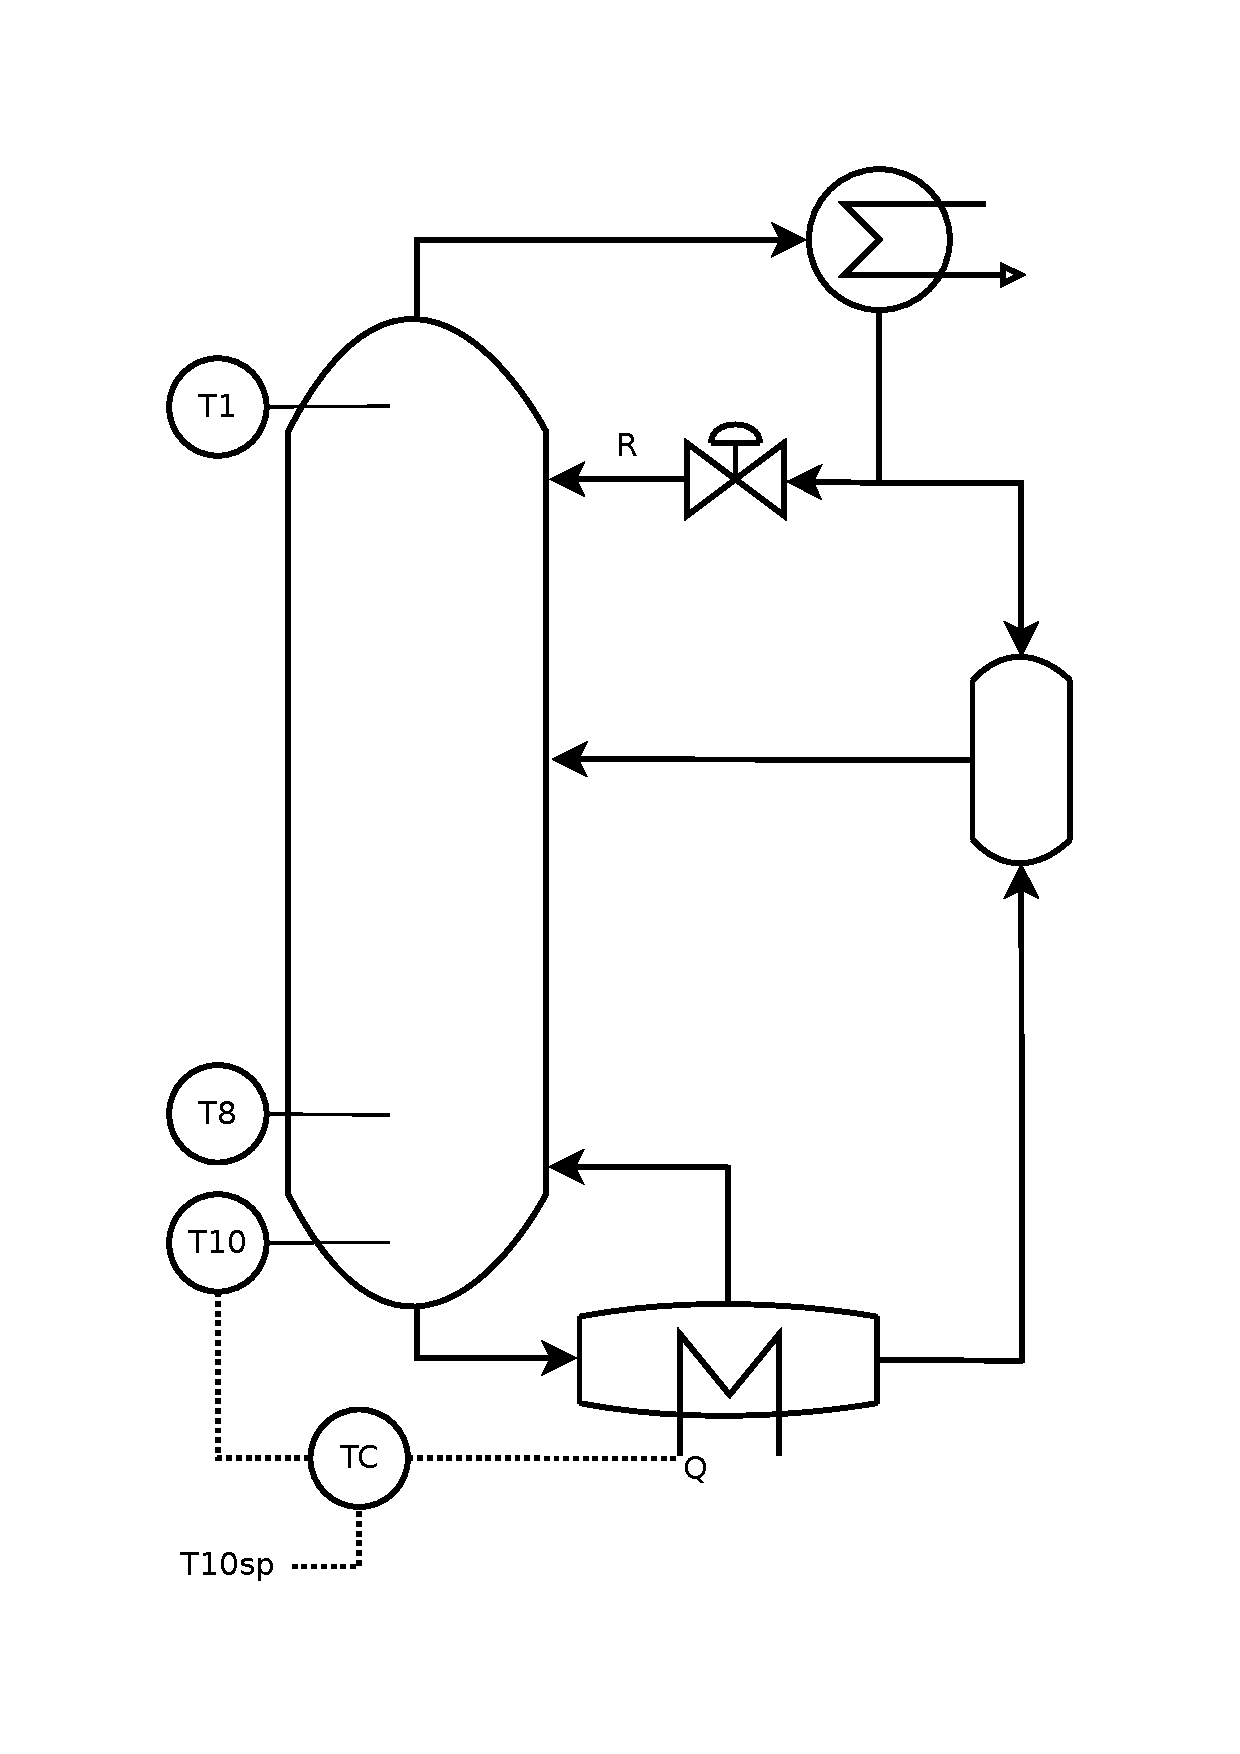
\includegraphics[width=8cm]{columnpfd.pdf}
  \caption[Laboratory distillation column photo and flow diagram]{Laboratory distillation column flow diagram.}
  \label{fig:columnpfd}
\end{figure}

The process model has been reduced to a $2\times2$ matrix.
Reflux flowrate ($R$, expressed as the milliamp signal sent to the control valve) and the setpoint of plate 10's temperature ($T_{10~sp}$) are the inputs, and the temperatures of plate 1 and 8 ($T_1\text{ \& }T_{8}$) are the outputs.
The temperature controller between $T_{10~sp}$ and $Q$ is part of the column's baselayer controls.
It was added as a safety measure, should the advanced control layer fail.

Equation~\ref{eq:columnmodel} shows the steady-state gain model ($G$) of the column.
\begin{equation}
  \label{eq:columnmodel}
                 % R      T10sp
  G = \bpm -0.0575 & 0.96 \\       % T1
           -0.146  & 0.518 \\ \epm % T8
\end{equation}

Table~\ref{tab:columnopcon} lists the operating conditions of the distillation column.
\begin{table}[htbp]
  \centering
  \begin{tabular}{llllll}
    \toprule
    \multicolumn{2}{c}{Variable} & \multicolumn{4}{c}{Constraints}\\
     && \multicolumn{2}{c}{Operating} & \multicolumn{2}{c}{Physical} \\
    \cmidrule(r){3-4} \cmidrule(r){5-6}
    && Low & High & Low & High \\ 
    \midrule
    Inputs &$R$ (mA)          & 11 & 15 & 4 & 20 \\
           &$T_{10~sp}$ (\textcelsius) & 78 & 82 & 25 & 90 \\[1.3ex]
    Outputs &$T_1$ (\textcelsius)     & 66 & 68 & 15 & 68 \\
            &$T_{8}$ (\textcelsius)   & 78 & 82 & 25 & 90 \\
    \bottomrule
  \end{tabular}
  \caption{Operating conditions of the laboratory distillation column.}
  \label{tab:columnopcon}
\end{table}

\subsection{Input and Output spaces}
From the data in table~\ref{tab:columnopcon} and equation~\ref{eq:columnmodel} the AIS and AOS of the laboratory distillation column can be generated as shown in figure~\ref{fig:columnaisaos}(a, b).
Take note that the operating limits for $R$, and the physical limits for $T_{10~sp}$ are used to construct the AIS.
The DOS, as described by the operating range of the outputs, is also shown in figure~\ref{fig:columnaisaos}(b, c).

\begin{figure}[htbp]
  \centering
    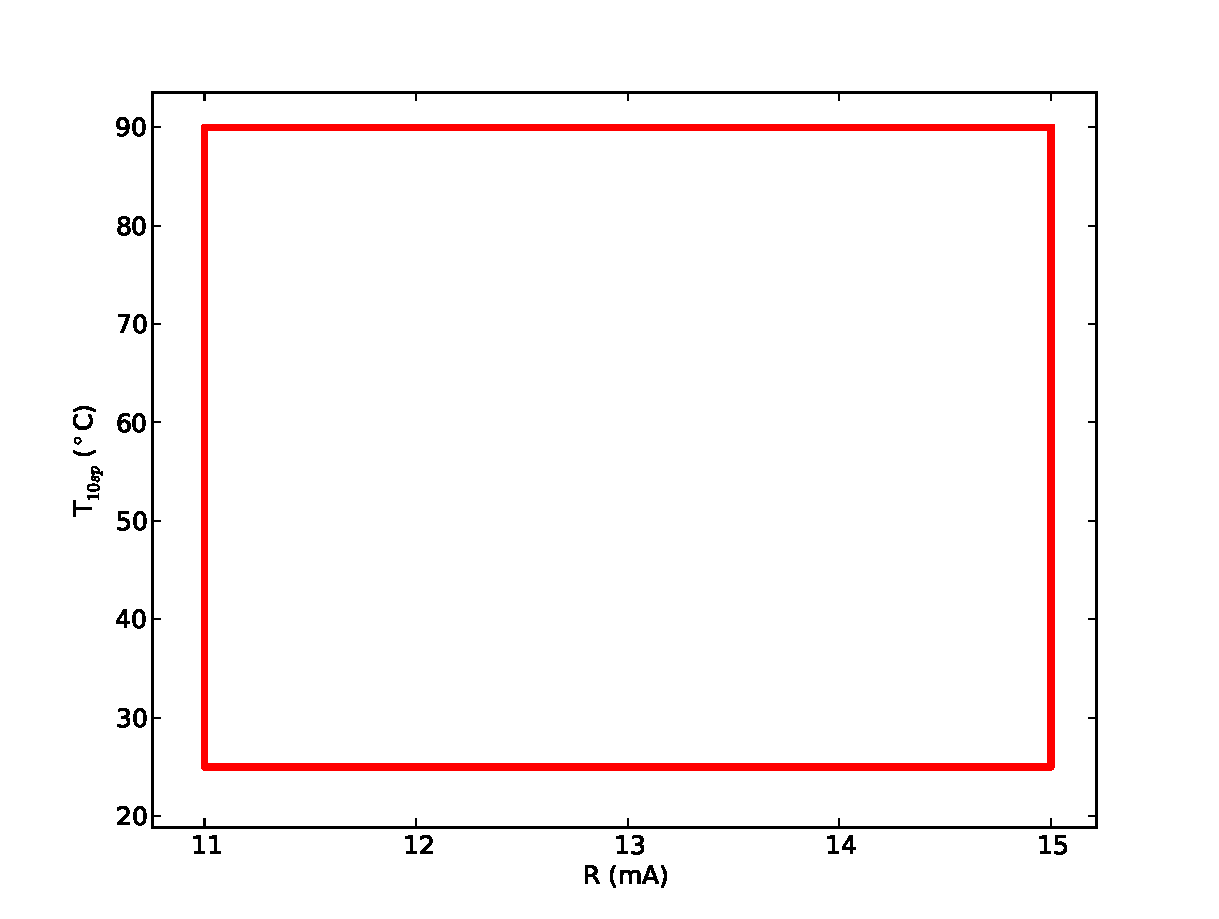
\includegraphics[width=8cm]{columnais.pdf}
    %\qquad
    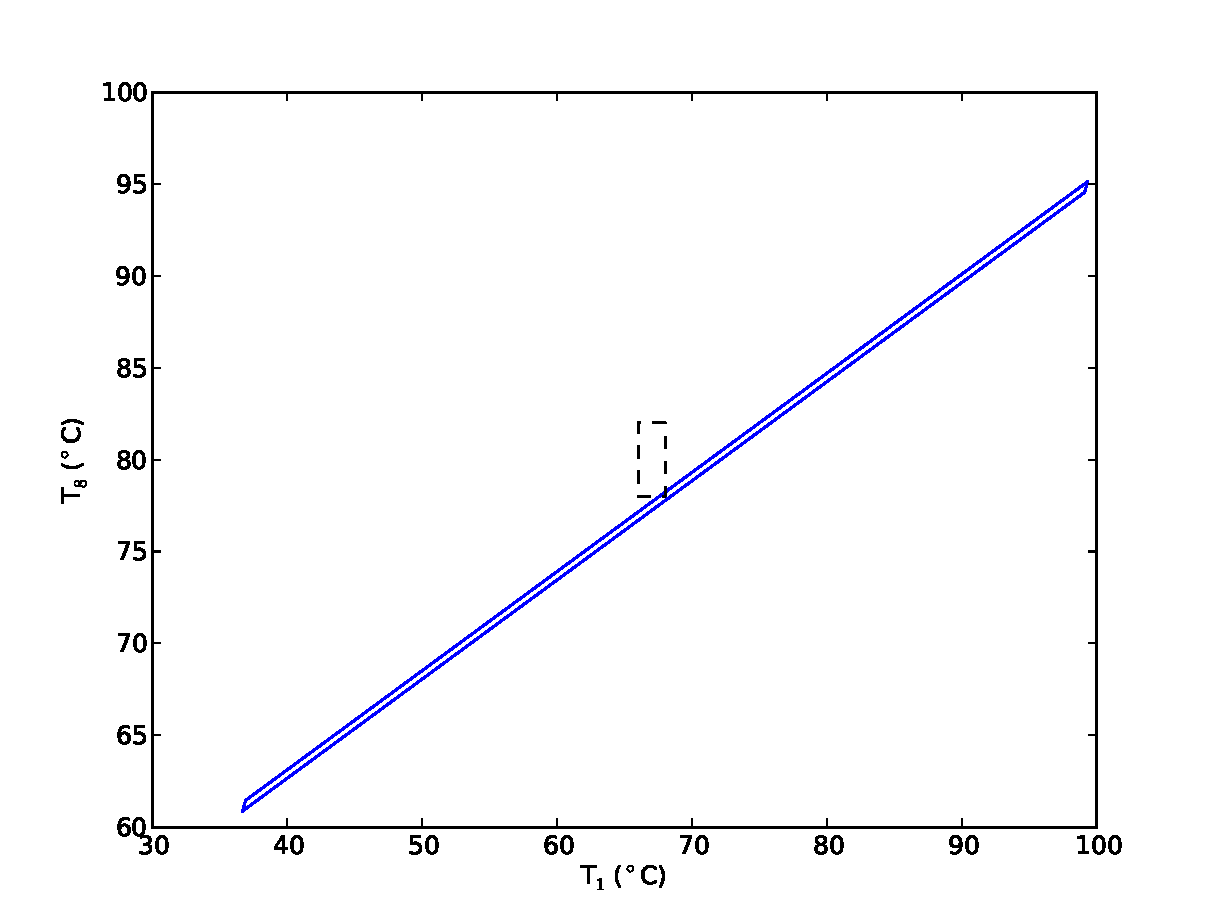
\includegraphics[width=8cm]{columnaos.pdf}
    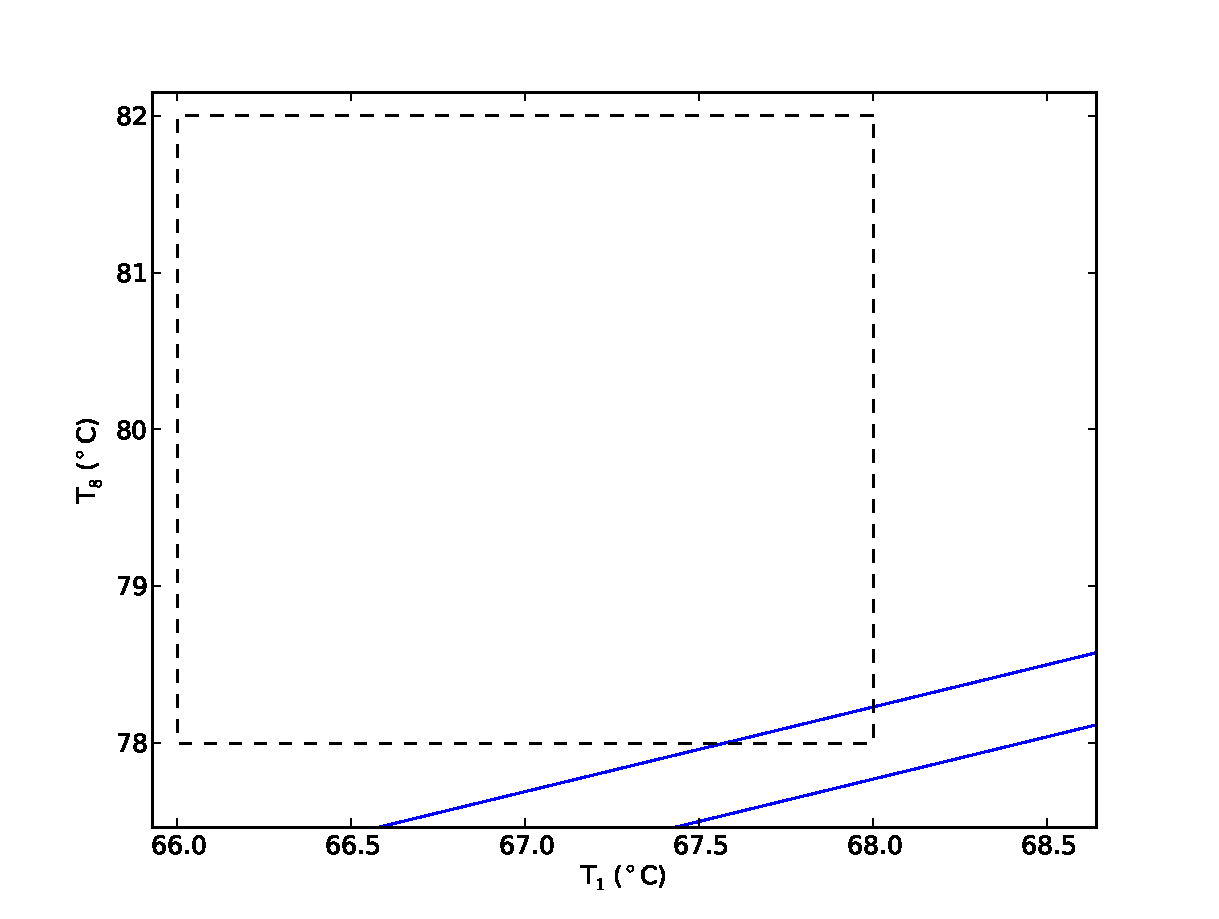
\includegraphics[width=8cm]{columnaosfocus.pdf}
  \caption{AIS (a), AOS and DOS (b), and AOS$\cap$DOS (c) showing a very small operating region.}
  \label{fig:columnaisaos}
\end{figure}

Figure~\ref{fig:columnaisaos}(c) focuses on the intersection of the AOS and the DOS.
The calculated OI is 0.006 which confirms that only a very small operating region within the DOS is attainable.
It is also clear that the upper limit of 82~\textcelsius\ on $T_8$ is unrealistic as the maximum value of $T_8$ (in the desired operating region) is only 78.2~\textcelsius.

\subsection{Constraint types}
The AIS of the distillation column consists of physical and operational constraints.
The small operating region necessitates the changing of input constraints to increase the process' operability, although the necessary changes are not immediately apparent.
For this reason it is important to identify the constraints that can be changed in the input space (i.e. non-hard, operational constraints) as well as their corresponding constraints in the output space.

The constraints on $R$ (figure~\ref{fig:columnaisaos}(a)) correspond to the long diagonal constraints in the output space (figure~\ref{fig:columnaisaos}(b)).
Therefore, changing the lower bound on $R$ will increase the Operability Index.
Decreasing the lower bound on $R$ to 4~mA increases the Operability Index to 0.125.

This highlights the importance of constraint and model interaction, as changing the limits on $T_{10~sp}$ (if this were possible) would have no effect on the process operability.

\subsection{Set fitting}
Returning to the original AOS/DOS intersection of figure~\ref{fig:columnaisaos}(b), it is advantageous to obtain a set of operating constraints that are fully feasible in both the input and output space.

\subsubsection{High and low limits}
A simple approach to obtain a set of feasible constraints is by fitting high and low limits within the AOS/DOS intersection.
Figure~\ref{fig:columnfitbox} shows the fitting of the largest set of this type as a dark dashed box.
 
\begin{figure}[htbp]
  \centering
    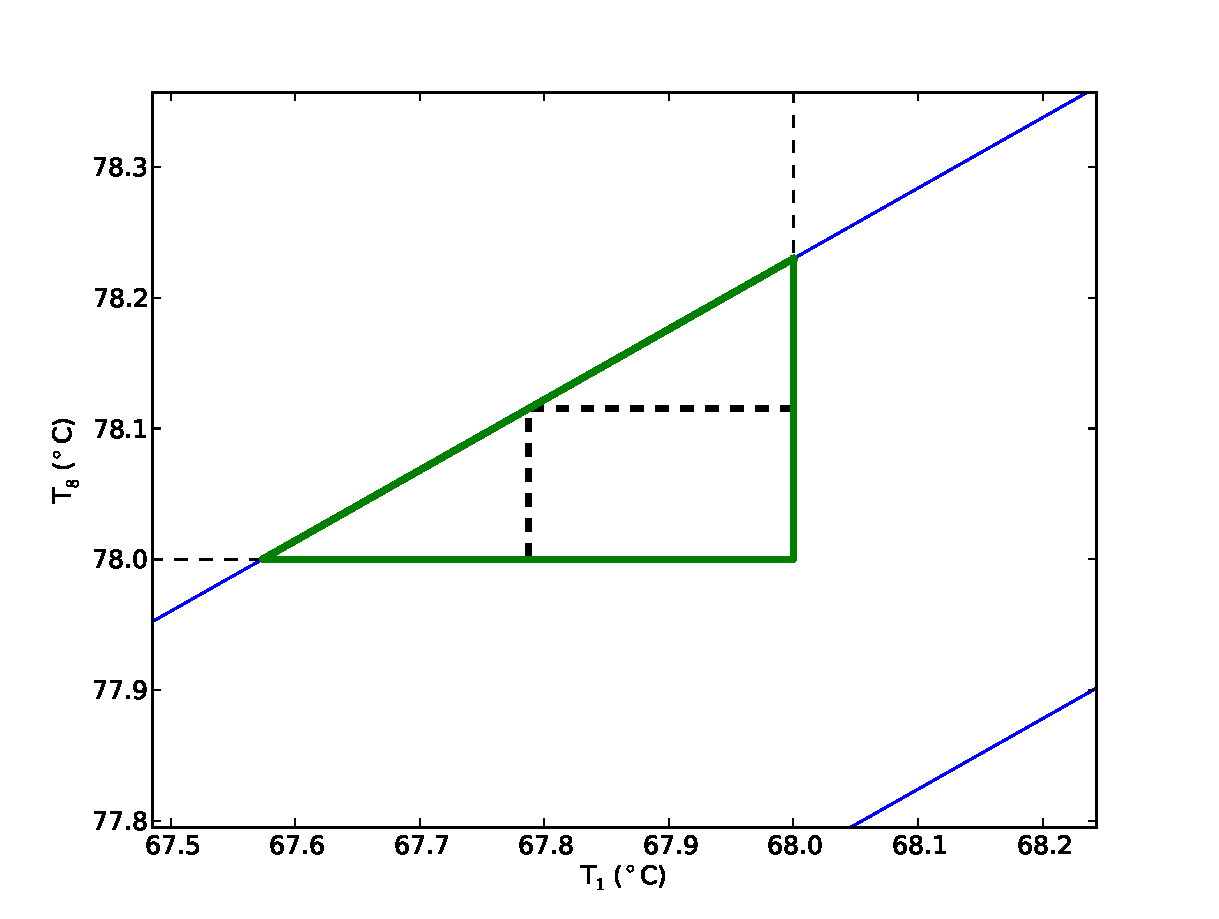
\includegraphics[width=8cm]{columnfitbox.pdf}
  \caption[Fitted constraints for the laboratory distillation column]{Intersection of AOS and DOS with fitted high and low limits for the column tray temperatures.}
  \label{fig:columnfitbox}
\end{figure}

This set is directly applicable to commercial MPC packages as only high and low limits on the original variables are present.
It can, however, be noted that only a fraction of the intersection is covered.
This problem worsens as the irregularity of the intersection increases.

\subsubsection{Constraint reformatting}
Rather than using the high and low limits shown in figure~\ref{fig:columnfitbox}, the constraints describing the whole intersection can be used to maximise the operating region.
This set of constraints need to be reformatted to be compatible with commercial MPC packages, as they only accept high and low limits on variables.

The dark triangle in figure~\ref{fig:columnfitbox} represents the constraints defining the intersection.
An unmeasured variable needs to be added to the process model to implement the diagonal constraint ($0.88T_8-0.47T_1\leq 36.56$~\textcelsius).
Naming the new output $y_1$ and augmenting the process model matrix as shown in equation~\ref{eq:columnnewmodel} allows for the diagonal (linear) constraint to be expressed simply as {$y_1~\leq~36.56$~\textcelsius}.
\begin{equation}
  \label{eq:columnnewmodel}
  G_{new}= \bpm -0.0575 & 0.96 \\       % T1
                  -0.146  & 0.518 \\      % T8
                   0.0956 & 1.30 \\ \epm  %y1
\end{equation}

\subsubsection{Set reduction}
When the intersection of the DOS and AOS contains many facets (as is typically the case for higher order systems), a large increase in model variables as well as constraints are needed to describe the complete intersection.

In this case, fitting a constraint set with fewer constraints than the original intersection, whilst still maximising the operational region, can be considered.
Whilst not illustrated in this paper, it is intuitive that the fraction of the intersection that will be covered is less than 1.
The set reduction procedure therefore becomes a trade-off between the operability obtained and the simplification of the control problem.

\subsection{Constraint changes}
It is typical of operators to change constraints during the operation of processes.
Usually, constraints are tightened on outputs or inputs.
It is intuitive that constraint tightening in the output space has a corresponding tightening effect in the input space, but the extent thereof isn't immediately clear.
The same reasoning applies to the changing of input constraints.

As an example, a change from the full intersection constraints to the fitted upper and lower bounds of figure~\ref{fig:columnfitbox} are considered and the effect of this constraint change in the input space investigated.
Figure~\ref{fig:columnconsinput}(a) shows the original AIS and DIS.
It is clear that the limits of the DOS -- now represented in the input space as the DIS -- are unattainable.

The effect of the constraint change is shown in figure~\ref{fig:columnconsinput}(b) as the transition from the dotted triangular constraint set to the parallelogram shaped dashed set.
From equation~\ref{eq:inputclamp} this corresponds to a 50\% clamping in the input space.

\begin{figure}[htbp]
  \centering
    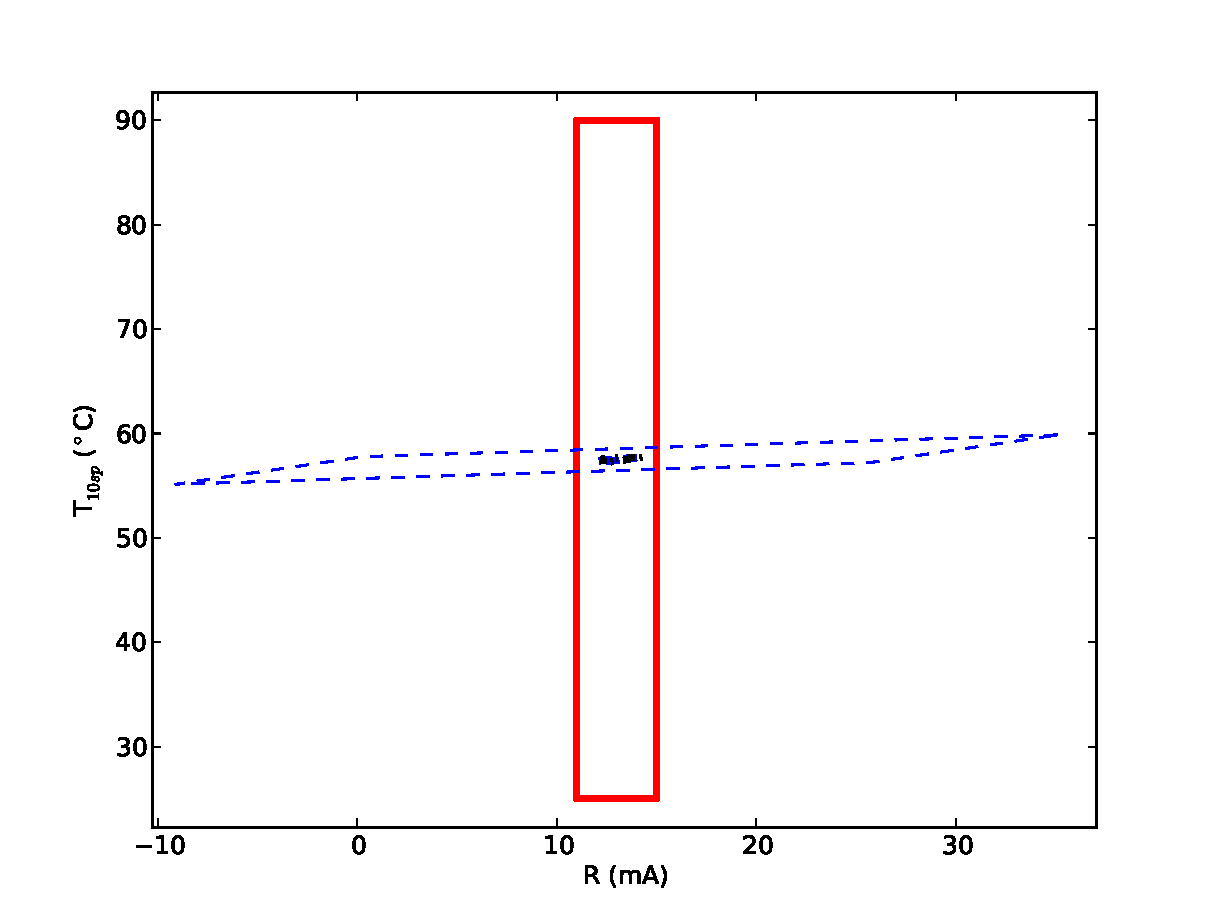
\includegraphics[width=8cm]{columninputs.pdf}
    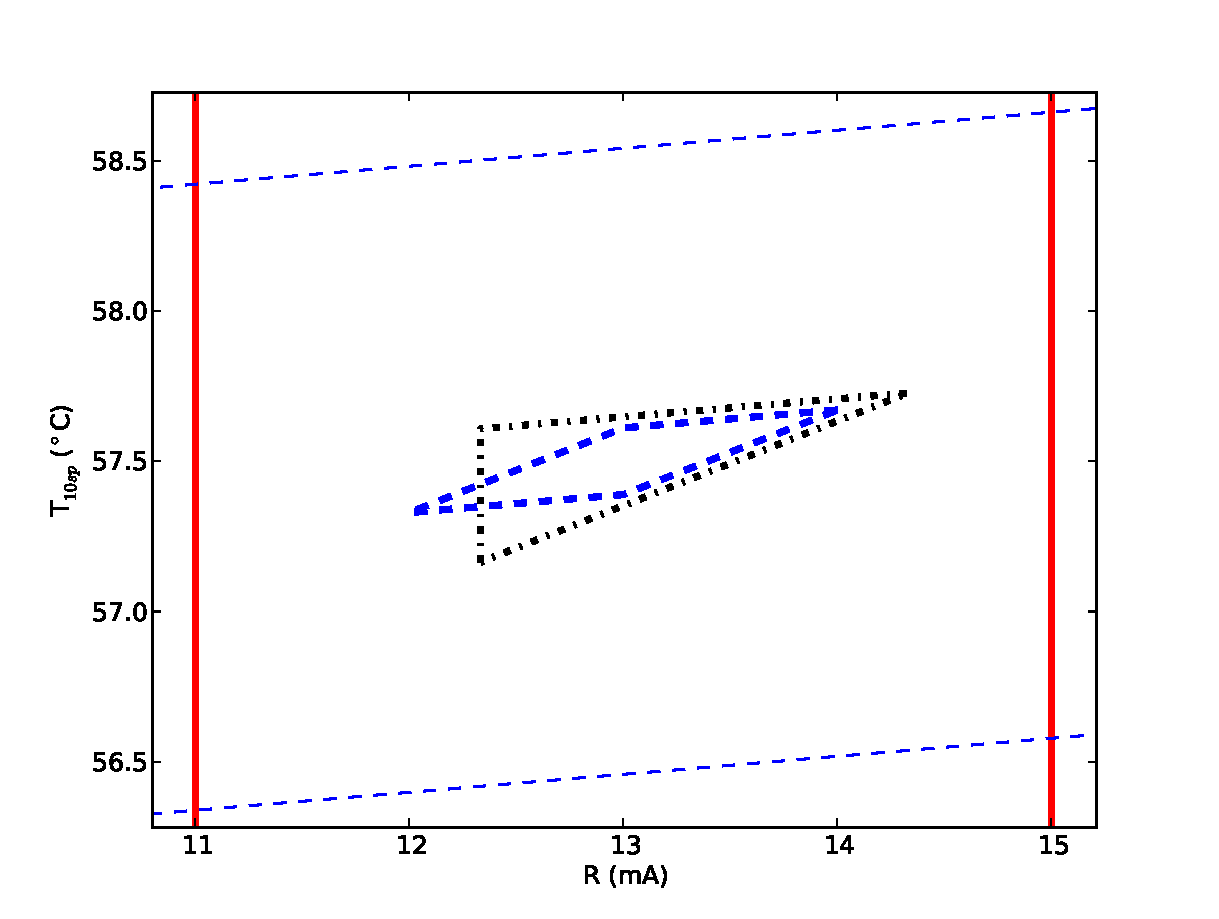
\includegraphics[width=8cm]{columninputszoom.pdf}
  \caption{Constraints in the input space for the column (a) and focus on the constraint changes showing input clamping (b).}
  \label{fig:columnconsinput}
\end{figure}

This figure also serves to confirm that the newly fitted constraints on the outputs correspond to a fully attainable region in the input space.


\subsection{MPC interfacing}
As with the level and flow rig, the operator interfaces (figures and ) are used to set the constraints for the system.
The modelling interfaces (figures and ) are used to augment the model for the addition of unmeasured variables.


\section{Conclusions}\label{sec:conclusions}
From the proposed method of systematic constraint handling and the illustrative example, a few conclusions can be drawn.
The results obtained by the method are readily applicable to commercial MPCs.

The specification of unrealistic constraints lead to a low Operability Index and unattainable expectations of both the inputs and outputs of the process.
Checking constraints via the process model can identify constraint sets that are not attainable.

Disambiguating the language used in specifying constraints, allow for identification of constraints that can be adjusted to increase process operability.
In the case of a process still in the design phase, the specific effect of constraints on variables can be used as a guide for possible design modifications. 

The constraints that describe the AOS/DOS intersection, represents the largest operating region for the given input and output constraints.
The constraints describing this intersection are usually linear combinations of variables and can be reformatted to conform to commercial MPC interfaces.
An unmeasured variable (resultant from the linear constraint) is added to the process model, and high and low constraints are imposed thereon.

The fitting of a constraint set within the AOS/DOS intersection leads to an operating region that is completely feasible in both the input and output space.
The size of a constraint set can be reduced by fitting a smaller set within, whilst maximising the operating region of the fitted set.
This reduces the control problem by reducing the number of active constraints on the system.

Finally, when constraint changes are made (during operation or design), checking changes to constraints via the process model allows for a measure of clamping to be determined.
This serves to inform operators of the resulting effect of changing constraints and guides design decisions.


%% ==== TAIL ====
\bibliographystyle{model4-names}
\bibliography{articlerefs}

\end{document}
